\section{\texttt{rpanel}}

\subsection*{Descrição}

%----------------------------------------------------------------------

\begin{frame}

  \texttt{rpanel} fornece um conjunto de funções para criar interfaces
  gráficas simples para controlar funções do R. As interfaces são
  contruídas usando o pacote \texttt{tcltk}. Além das funções que
  fornecem elementos de interface, o pacote tem funções para interfaces
  específicas chamadas de \emph{cartoons}.

  \begin{itemize}
  \item Autores: Bowman, Bowman, Gibson and Crawford
  \item Lançamento: 21-Aug-2006
  \item Versão: 1.1-3
  \item URL:
    \url{http://cran.r-project.org/web/packages/rpanel/index.html}
\end{itemize}

\end{frame}

\begin{frame}

\begin{itemize}
\item Alguns pacotes baseados em \texttt{rpanel}:
  \href{http://cran.r-project.org/web/packages/GUIDE/index.html}{\texttt{GUIDE}},
  \href{http://cran.r-project.org/web/packages/MDSGUI/index.html}{\texttt{MDSGUI}},
  \href{http://cran.r-project.org/web/packages/RVideoPoker/index.html}{\texttt{RVideoPoker}},
  \href{https://github.com/walmes/wzRfun/blob/master/R/rp.nls.R}{\texttt{wzRfun::rp.nls}}.
  e mais.
\end{itemize}

\end{frame}

%----------------------------------------------------------------------

\subsection*{Como usar}

\begin{frame}
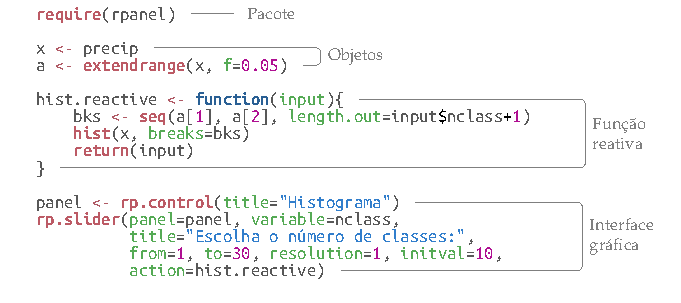
\includegraphics[scale=1]{./tikz/hist_slider_rpanel-1.pdf}
\end{frame}

\begin{frame}
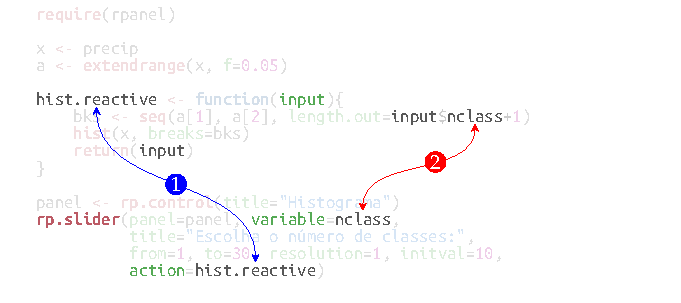
\includegraphics[scale=1]{./tikz/hist_slider_rpanel-2.pdf}
\end{frame}

%----------------------------------------------------------------------

\subsection*{Exemplos}

\begin{frame}
 Praticando:
  \begin{enumerate}
  \item
    \href{run:./R/rpanel/rpanel.R}{R Script rpanel}
  \item 
	\href{run:rpanel.html}{Galeria rpanel IGUIR}
  \end{enumerate}

  \vspace{0.5cm}
  Algumas aplicações com o rpanel:
  \begin{itemize}
  \item \href{http://www.stats.gla.ac.uk/~adrian/rpanel/}{Galeria
      do autor},
  \item \href{http://www.r-bloggers.com/?s=rpanel}{Busca no R
      Bloggers}
  \end{itemize}

\end{frame}
